%%%%%%%%%%%%%%%%%%%%%%%%%%%%%%%%%%%%
% Lesson Plan (50 minutes)
%%%%%%%%%%%%%%%%%%%%%%%%%%%%%%%%%%%%
\begin{frame}
    \frametitle{Lesson Plan}
    \begin{itemize}
        \item xx min Lecture: Motivate hypothesis tests
        \item xx min Lecture: Hypothesis testing framework
        \item xx min Lecture: Tying in confidence intervals
        \item xx min Lecture: Decision errors, error table
        \item xx min R Demonstration: examples of hypothesis tests and decision errors
        \begin{enumerate}
            \item Highlight: an error that might be easy to make in their own work
        \end{enumerate}
        \item xx min R Demonstration: computing error rates
        \item xx min Edfinity quiz: decision errors, HT concept check
        \item xx min Lecture: introduce test statistics (to be continued next time)
    \end{itemize}
\end{frame}
            
%%%%%%%%%%%%%%%%%%%%%%%%%%%%%%%%%%%%
% Learning objectives:
%%%%%%%%%%%%%%%%%%%%%%%%%%%%%%%%%%%%
\begin{frame}
    \frametitle{Learning Objectives}
    \begin{itemize}
        \item \textbf{M3, LO4: Explain Hypothesis Testing and Its Limitations:} Discuss the use cases and potential issues with hypothesis testing, including the interpretation of results.
        \item \textbf{M3, LO5: Understand Errors and Significance Levels:} Identify Type I and Type II errors and explain how they are influenced by changes in the significance level.
        \item \textbf{M4, LO2: Design and Interpret Confidence Intervals:} Design, execute, and interpret confidence intervals for the population proportion.
        \item \textbf{M4, LO3: Conduct and Interpret Hypothesis Tests for Proportions:} Design, execute, and interpret hypothesis tests for population proportions.
    \end{itemize}
\end{frame}
    
%%%%%%%%%%%%%%%%%%%%%%%%%%%%%%%%%%%%
% TODO: Copy and adapt these slides base on the lesson plan
%%%%%%%%%%%%%%%%%%%%%%%%%%%%%%%%%%%%

\section{Hypothesis testing for a proportion}

%%%%%%%%%%%%%%%%%%%%%%%%%%%%%%%%%%%%

\subsection{Hypothesis testing framework}

%%%%%%%%%%%%%%%%%%%%%%%%%%%%%%%%%%%%

\begin{frame}
\frametitle{Remember when...}

Gender discrimination experiment:

{\footnotesize
\begin{tabular}{ll  cc c} 
  		&				& \multicolumn{2}{c}{\textit{Promotion}} \\
\cline{3-4}
							&			& Promoted	& Not Promoted 	& Total	\\
\cline{2-5}
\multirow{2}{*}{\textit{Gender	}}	&Male 		& 21	 	& 3		& 24 	\\
							&Female		& 14	 	& 10 	 	& 24 \\
\cline{2-5}
							&Total		& 35		& 13		& 48 \\
\end{tabular}
}

\pause

\[ \hat{p}_{males} = 21 / 24 \approx 0.88 ~ \text{ and } ~ \hat{p}_{females} = 14 / 24 \approx 0.58 \]

\pause

Possible explanations:
\begin{itemize}
\item Promotion and gender are \hl{independent}, no gender discrimination, observed difference in proportions is simply due to chance. $\rightarrow$ \orange{null} - {\small (nothing is going on)}
\item Promotion and gender are \hl{dependent}, there is gender discrimination, observed difference in proportions is not due to chance. $\rightarrow$ \orange{alternative} - {\small (something is going on)}

\end{itemize}

\end{frame}

%%%%%%%%%%%%%%%%%%%%%%%%%%%%%%%%%%%%

\begin{frame}
\frametitle{Result}

\begin{center}
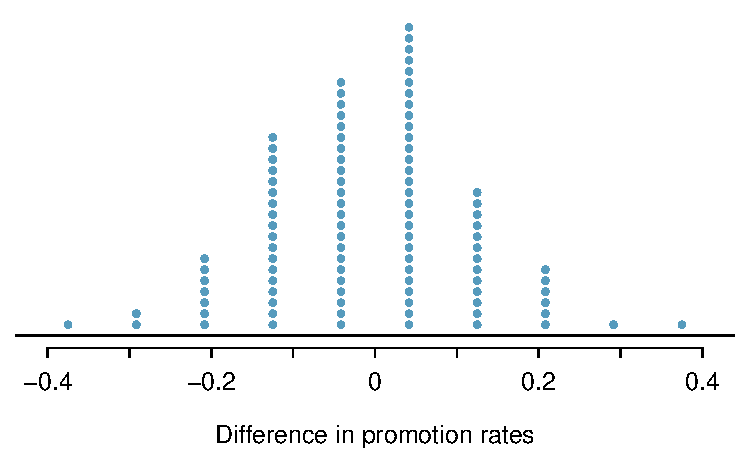
\includegraphics[width=0.75\textwidth]{5-3_ht_prop/figures/discRandDotPlot/discRandDotPlot}
\end{center}

\pause

Since it was quite unlikely to obtain results like the actual data or something more extreme in the simulations (male promotions being 30\% or more higher than female promotions), we decided to reject the null hypothesis in favor of the alternative.

\end{frame}

%%%%%%%%%%%%%%%%%%%%%%%%%%%%%%%%%%%%

\begin{frame}
\frametitle{Recap: hypothesis testing framework}

\begin{itemize}
\item We start with a \hl{null hypothesis ($H_0$)} that represents the status quo.
\pause
\item We also have an \hl{alternative hypothesis ($H_A$)} that represents our research question, i.e. what we're testing for.
\pause
\item We conduct a hypothesis test under the assumption that the null hypothesis is true, either via simulation or traditional methods based on the central limit theorem (coming up next...).
\pause
\item If the test results suggest that the data do not provide convincing evidence for the alternative hypothesis, we stick with the null hypothesis. If they do, then we reject the null hypothesis in favor of the alternative.
\end{itemize}
\pause
We'll formally introduce the hypothesis testing framework using an example on testing a claim about a proportion.

\end{frame}

%%%%%%%%%%%%%%%%%%%%%%%%%%%%%%%%%%%

 \subsection{Testing hypotheses using confidence intervals} 
 
%%%%%%%%%%%%%%%%%%%%%%%%%%%%%%%%%%%%
 
\begin{frame}
\frametitle{Testing hypotheses using confidence intervals}
 
{\small \dq{Earlier we calculated a 95\% confidence interval for the proporton of American Facebook users who think Facebook categorizes their interests accurately as 64\% to 67\%. Based on this confidence interval, do the data support the hypothesis that majority of American Facebook users think Facebook categorizes their interests accurately.}}
 
\pause
 
\begin{itemize}
 
\item The associated hypotheses are:
\begin{itemize}
\item[$H_0$:] $p = 0.50$: 50\% of American Facebook users think Facebook categorizes their interests accurately
\item[$H_A$:] $p > 0.50$: More than 50\% of American Facebook users think Facebook categorizes their interests accurately
\end{itemize}
 
\pause
 
\item Null value is not included in the interval $\rightarrow$ reject the null hypothesis.
 
\pause
 
\item This is a quick-and-dirty approach for hypothesis testing, but it doesn't tell us the likelihood of certain outcomes under the null hypothesis (p-value).
 
\end{itemize}
 
\end{frame}
 
%%%%%%%%%%%%%%%%%%%%%%%%%%%%%%%%%%%%

\subsection{Decision errors}

%%%%%%%%%%%%%%%%%%%%%%%%%%%%%%%%%%%%

\begin{frame}
\frametitle{Decision errors}

\begin{itemize}

\item Hypothesis tests are not flawless.

\item In the court system innocent people are sometimes wrongly convicted and the guilty sometimes walk free.

\item Similarly, we can make a wrong decision in statistical hypothesis tests as well. 

\item The difference is that we have the tools necessary to quantify how often we make errors in statistics.

\end{itemize}

\end{frame}

%%%%%%%%%%%%%%%%%%%%%%%%%%%%%%%%%%%%
 
\begin{frame}
\frametitle{Decision errors (cont.)}

There are two competing hypotheses: the null and the alternative. In a hypothesis test, we make a decision about which might be true, but our choice might be incorrect. \\

\pause

\begin{center}
\begin{tabular}{l l | c c}
\multicolumn{2}{c}{} & \multicolumn{2}{c}{\textbf{Decision}} \\
& & fail to reject $H_0$ &  reject $H_0$ \\
  \cline{2-4}
& $H_0$ true & \onslide<3->{\green{$\checkmark$}} &  \onslide<5->{\orange{Type 1 Error}} \\
\raisebox{1.5ex}{\textbf{Truth}} & $H_A$ true & \onslide<6->{\orange{Type 2 Error}} & \onslide<4->{\green{$\checkmark$}} \\
  \cline{2-4}
\end{tabular}
\end{center}

\begin{itemize}
\item \onslide<5->{A \hl{Type 1 Error} is rejecting the null hypothesis when $H_0$ is true.}

\item \onslide<6->{A \hl{Type 2 Error} is failing to reject the null hypothesis when $H_A$ is true.}

\item \onslide<7->{We (almost) never know if $H_0$ or $H_A$ is true, but we need to consider all possibilities.}

\end{itemize}

\end{frame}

%%%%%%%%%%%%%%%%%%%%%%%%%%%%%%%%%%%%

\begin{frame}[shrink]
\frametitle{Hypothesis Test as a trial}

If we again think of a hypothesis test as a criminal trial then it makes sense to frame the verdict in terms of the null and alternative hypotheses:
\begin{align*}
H_0&:\text{ Defendant is innocent} \\
H_A&:\text{ Defendant is guilty}
\end{align*}

Which type of error is being committed in the following circumstances?

\begin{itemize}
\item Declaring the defendant innocent when they are actually guilty
\soln{\only<2->{\begin{center}\hl{Type 2 error}\end{center}}}
\item Declaring the defendant guilty when they are actually innocent
\soln{\only<3->{\begin{center}\hl{Type 1 error}\end{center}}}
\end{itemize}

\only<4->{Which error do you think is the worse error to make?}
\only<5>{\begin{center}{\footnotesize ``better that ten guilty persons escape than that one innocent suffer''\\ -- William Blackstone}\end{center}}
\end{frame}

%%%%%%%%%%%%%%%%%%%%%%%%%%%%%%%%%%%%

\begin{frame}
\frametitle{Type 1 error rate}

\begin{itemize}

\item As a general rule we reject $H_0$ when the p-value is less than 0.05, i.e. we use a \hl{significance level} of 0.05, \mathhl{\alpha = 0.05}.

\pause

\item This means that, for those cases where $H_0$ is actually true, we do not want to incorrectly reject it more than 5\% of those times. 

\pause

\item In other words, when using a 5\% significance level there is about 5\% chance of making a Type 1 error if the null hypothesis is true.
\[ \mathhl{ P(\text{Type 1 error | $H_0$ true}) = \alpha } \]

\pause

\item This is why we prefer small values of $\alpha$ -- increasing $\alpha$ increases the Type 1 error rate.

\end{itemize}

\end{frame}

%%%%%%%%%%%%%%%%%%%%%%%%%%%%%%%%%%%%

\subsection{Formal testing using p-values}

%%%%%%%%%%%%%%%%%%%%%%%%%%%%%%%%%%%%

\begin{frame}
\frametitle{Facebook interest categories}
 
\dq{ The same survey asked the 850 respondents how comfortable they are with Facebook creating a list of categories for them. 41\% of the respondents said they are comfortable. Do these data provide convincing evidence that the proportion of American Facebook users are comfortable with Facebook creating a list of interest categories for them is different than 50\%?}
 
\vfill
 
\ct{\webURL{https://www.pewinternet.org/2019/01/16/facebook-algorithms-and-personal-data/}}
 
\end{frame}
 
%%%%%%%%%%%%%%%%%%%%%%%%%%%%%%%%%%

\begin{frame}
\frametitle{Setting the hypotheses}

\begin{itemize}

\item The \hl{parameter of interest} is the proportion of \underline{all} American Facebook users who are comfortable with Facebook creating categories of interests for them.

\pause

\item There may be two explanations why our sample proportion is lower than 0.50 (minority).
\begin{itemize}
\item The true population proportion is different than 0.50.
\item The true population mean is 0.50, and the difference between the true population proportion and the sample proportion is simply due to natural sampling variability.
\end{itemize}

 \end{itemize}

\end{frame}

%%%%%%%%%%%%%%%%%%%%%%%%%%%%%%%%%%
 
\begin{frame}
\frametitle{Setting the hypotheses}

\begin{itemize}

\item We start with the assumption that 50\% of American Facebook users are comfortable with Facebook creating categories of interests for them
\[ \mathhl{H_0:}~p = 0.50 \]

\pause

\item We test the claim that the proportion of American Facebook users who are comfortable with Facebook creating categories of interests for them is different than 50\%
\[ \mathhl{H_A:}~p \ne 0.50 \]

\end{itemize}

\end{frame}

%%%%%%%%%%%%%%%%%%%%%%%%%%%%%%%%%

\begin{frame}
\frametitle{Facebook interest categories - conditions}

\pq{Which of the following is \emph{not} a condition that needs to be met to proceed with this hypothesis test?}

\begin{enumerate}[(a)]
\item Respondents in the sample should be independent of each other with respect to whether or not they feel comfortable with their interests being categorized by Facebook.
\item Sampling should have been done randomly.
\item The sample size should be less than 10\% of the population of all American Facebook users.
\solnMult{ There should be at least 30 respondents in the sample.}
\item There should be at least 10 expected successes and 10 expected failure.
\end{enumerate}

\end{frame}

%%%%%%%%%%%%%%%%%%%%%%%%%%%%%%%%%
 
\begin{frame}
\frametitle{Test statistic}
 
In order to evaluate if the observed sample mean is unusual for the hypothesized sampling distribution, we determine how many standard errors away from the null it is, which is also called the \hl{test statistic}.
 
\pause
 
\[ \hat{p} \sim N \pr{ \mu = 0.50, SE = \sqrt{\frac{0.50 \times 0.50}{850} }  } \]

\pause

\[ Z = \frac{0.41 - 0.50}{0.0171} = -5.26 \]
 
 \pause
 
\dq{The sample proportion is 5.26 standard errors away from the hypothesized value. Is this considered unusually low? That is, is the result \hl{statistically significant}?}
 
\pause
 
\soln{Yes, and we can quantify how unusual it is using a p-value.}
 
\end{frame}
 
%%%%%%%%%%%%%%%%%%%%%%%%%%%%%%%%%%

\begin{frame}
\frametitle{p-values}

\begin{itemize}

\item We then use this test statistic to calculate the \hl{p-value}, the probability of observing data at least as favorable to the alternative hypothesis as our current data set, if the null hypothesis were true.

\pause

\item If the p-value is \hl{low} (lower than the significance level, $\alpha$, which is usually 5\%) we say that it would be very unlikely to observe the data if the null hypothesis were true, and hence \hl{reject $H_0$}.

\pause

\item If the p-value is \hl{high} (higher than $\alpha$) we say that it is likely to observe the data even if the null hypothesis were true, and hence \hl{do not reject $H_0$}.

\end{itemize}

\end{frame}

%%%%%%%%%%%%%%%%%%%%%%%%%%%%%%%%%%%%

\begin{frame}
\frametitle{Facebook interest categories - p-value}

\hl{p-value:} probability of observing data at least as favorable to $H_A$ as our current data set (a sample proportion lower than 0.41), if in fact $H_0$ were true (the true population proportion was 0.50).

\pause

\[ P(\hat{p} < 0.41~\text{ or }~\hat{p} > 0.59~|~p = 0.50) = P(|Z| > 5.26) < 0.0001 \]

\end{frame}

%%%%%%%%%%%%%%%%%%%%%%%%%%%%%%%%%

\begin{frame}
\frametitle{Facebook interest categories - Making a decision}

\begin{itemize}

\item p-value $<$ 0.0001

\pause

\begin{itemize}
\item If 50\% of all American FB users are comfortable with FB creating these interest categories, there is less than a 0.01\% chance of observing a random sample of 850 American Facebook users where 41\% or fewer or 59\% of higher feel comfortable with it.
\pause
\item Pretty low probability to think that observed sample proportion, or something more extreme, is likely to happen by chance.
\end{itemize}

\pause
\item Since p-value is \orange{low} (lower than 5\%) we \orange{reject $H_0$}.

\pause
\item The data provide convincing evidence that the proportion of American FB users who are comfortable with FB creating a list of interest categories for them is different than 50\%.

\pause
\item The difference between the null value of 0.50 and observed sample proportion of 0.41 is \orange{not due to chance} or sampling variability.

\end{itemize}

\end{frame}

%%%%%%%%%%%%%%%%%%%%%%%%%%%%%%%%%%%

\subsection{Choosing a significance level}

%%%%%%%%%%%%%%%%%%%%%%%%%%%%%%%%%%%%

\begin{frame}
\frametitle{Choosing a significance level}

\begin{itemize}

\item While the the traditional level is 0.05, it is helpful to adjust the significance level based on the application. 

\item Select a level that is smaller or larger than 0.05 depending on the consequences of any conclusions reached from the test.

\item If making a Type 1 Error is dangerous or especially costly, we should choose a small significance level (e.g. 0.01). Under this scenario we want to be very cautious about rejecting the null hypothesis, so we demand very strong evidence favoring $H_A$ before we would reject $H_0$.

\item If a Type 2 Error is relatively more dangerous or much more costly than a Type 1 Error, then we should choose a higher significance level (e.g. 0.10). Here we want to be cautious about failing to reject $H_0$ when the null is actually false.

\end{itemize}

\end{frame}

%%%%%%%%%%%%%%%%%%%%%%%%%%%%%%%%%%%%
 
\subsection{One vs. two sided hypothesis tests}
 
%%%%%%%%%%%%%%%%%%%%%%%%%%%%%%%%%%%%
 
\begin{frame}
\frametitle{One vs. two sided hypothesis tests}
 
\begin{itemize}
 
\item In two sided hypothesis tests we are interested in whether $p$ is either above or below some null value $p_0$: $H_A: p \ne p_0$.
 
\item In one sided hypothesis tests we are interested in $p$ differing from the null value $p_0$ in one direction (and not the other):
\begin{itemize}
\item If there is only value in detecting if population parameter is less than $p_0$, then $H_A: p < p_0$.
\item If there is only value in detecting if population parameter is greater than $p_0$, then $H_A: p > p_0$.
\end{itemize}

\item Two-sided tests are often more appropriate as we often want to detect if the data goes clearly in the opposite direction of our alternative hypothesis as well.

\end{itemize}

\end{frame}

%%%%%%%%%%%%%%%%%%%%%%%%%%%%%%%%%%%%
 

    